\documentclass[8pt,ignorenonframetext,dvipsnames]{beamer}
\setbeamertemplate{caption}[numbered]
\setbeamertemplate{caption label separator}{: }
\setbeamercolor{caption name}{fg=normal text.fg}
\beamertemplatenavigationsymbolsempty
\usepackage{lmodern}
\usepackage{amssymb,amsmath}
\usepackage{ifxetex,ifluatex}
\usepackage{fixltx2e} % provides \textsubscript
\ifnum 0\ifxetex 1\fi\ifluatex 1\fi=0 % if pdftex
  \usepackage[T1]{fontenc}
  \usepackage[utf8]{inputenc}
\else % if luatex or xelatex
  \ifxetex
    \usepackage{mathspec}
  \else
    \usepackage{fontspec}
  \fi
  \defaultfontfeatures{Ligatures=TeX,Scale=MatchLowercase}
\fi
% use upquote if available, for straight quotes in verbatim environments
\IfFileExists{upquote.sty}{\usepackage{upquote}}{}
% use microtype if available
\IfFileExists{microtype.sty}{%
\usepackage{microtype}
\UseMicrotypeSet[protrusion]{basicmath} % disable protrusion for tt fonts
}{}
\newif\ifbibliography
\hypersetup{
            pdftitle={Managing and Manipulating Data Using R},
            pdfauthor={Ozan Jaquette},
            pdfborder={0 0 0},
            breaklinks=true}
\urlstyle{same}  % don't use monospace font for urls
\usepackage{color}
\usepackage{fancyvrb}
\newcommand{\VerbBar}{|}
\newcommand{\VERB}{\Verb[commandchars=\\\{\}]}
\DefineVerbatimEnvironment{Highlighting}{Verbatim}{commandchars=\\\{\}}
% Add ',fontsize=\small' for more characters per line
\usepackage{framed}
\definecolor{shadecolor}{RGB}{248,248,248}
\newenvironment{Shaded}{\begin{snugshade}}{\end{snugshade}}
\newcommand{\KeywordTok}[1]{\textcolor[rgb]{0.13,0.29,0.53}{\textbf{#1}}}
\newcommand{\DataTypeTok}[1]{\textcolor[rgb]{0.13,0.29,0.53}{#1}}
\newcommand{\DecValTok}[1]{\textcolor[rgb]{0.00,0.00,0.81}{#1}}
\newcommand{\BaseNTok}[1]{\textcolor[rgb]{0.00,0.00,0.81}{#1}}
\newcommand{\FloatTok}[1]{\textcolor[rgb]{0.00,0.00,0.81}{#1}}
\newcommand{\ConstantTok}[1]{\textcolor[rgb]{0.00,0.00,0.00}{#1}}
\newcommand{\CharTok}[1]{\textcolor[rgb]{0.31,0.60,0.02}{#1}}
\newcommand{\SpecialCharTok}[1]{\textcolor[rgb]{0.00,0.00,0.00}{#1}}
\newcommand{\StringTok}[1]{\textcolor[rgb]{0.31,0.60,0.02}{#1}}
\newcommand{\VerbatimStringTok}[1]{\textcolor[rgb]{0.31,0.60,0.02}{#1}}
\newcommand{\SpecialStringTok}[1]{\textcolor[rgb]{0.31,0.60,0.02}{#1}}
\newcommand{\ImportTok}[1]{#1}
\newcommand{\CommentTok}[1]{\textcolor[rgb]{0.56,0.35,0.01}{\textit{#1}}}
\newcommand{\DocumentationTok}[1]{\textcolor[rgb]{0.56,0.35,0.01}{\textbf{\textit{#1}}}}
\newcommand{\AnnotationTok}[1]{\textcolor[rgb]{0.56,0.35,0.01}{\textbf{\textit{#1}}}}
\newcommand{\CommentVarTok}[1]{\textcolor[rgb]{0.56,0.35,0.01}{\textbf{\textit{#1}}}}
\newcommand{\OtherTok}[1]{\textcolor[rgb]{0.56,0.35,0.01}{#1}}
\newcommand{\FunctionTok}[1]{\textcolor[rgb]{0.00,0.00,0.00}{#1}}
\newcommand{\VariableTok}[1]{\textcolor[rgb]{0.00,0.00,0.00}{#1}}
\newcommand{\ControlFlowTok}[1]{\textcolor[rgb]{0.13,0.29,0.53}{\textbf{#1}}}
\newcommand{\OperatorTok}[1]{\textcolor[rgb]{0.81,0.36,0.00}{\textbf{#1}}}
\newcommand{\BuiltInTok}[1]{#1}
\newcommand{\ExtensionTok}[1]{#1}
\newcommand{\PreprocessorTok}[1]{\textcolor[rgb]{0.56,0.35,0.01}{\textit{#1}}}
\newcommand{\AttributeTok}[1]{\textcolor[rgb]{0.77,0.63,0.00}{#1}}
\newcommand{\RegionMarkerTok}[1]{#1}
\newcommand{\InformationTok}[1]{\textcolor[rgb]{0.56,0.35,0.01}{\textbf{\textit{#1}}}}
\newcommand{\WarningTok}[1]{\textcolor[rgb]{0.56,0.35,0.01}{\textbf{\textit{#1}}}}
\newcommand{\AlertTok}[1]{\textcolor[rgb]{0.94,0.16,0.16}{#1}}
\newcommand{\ErrorTok}[1]{\textcolor[rgb]{0.64,0.00,0.00}{\textbf{#1}}}
\newcommand{\NormalTok}[1]{#1}
\usepackage{longtable,booktabs}
\usepackage{caption}
% These lines are needed to make table captions work with longtable:
\makeatletter
\def\fnum@table{\tablename~\thetable}
\makeatother
\usepackage{graphicx,grffile}
\makeatletter
\def\maxwidth{\ifdim\Gin@nat@width>\linewidth\linewidth\else\Gin@nat@width\fi}
\def\maxheight{\ifdim\Gin@nat@height>\textheight0.8\textheight\else\Gin@nat@height\fi}
\makeatother
% Scale images if necessary, so that they will not overflow the page
% margins by default, and it is still possible to overwrite the defaults
% using explicit options in \includegraphics[width, height, ...]{}
\setkeys{Gin}{width=\maxwidth,height=\maxheight,keepaspectratio}

% Prevent slide breaks in the middle of a paragraph:
\widowpenalties 1 10000
\raggedbottom

\AtBeginPart{
  \let\insertpartnumber\relax
  \let\partname\relax
  \frame{\partpage}
}
\AtBeginSection{
  \ifbibliography
  \else
    \let\insertsectionnumber\relax
    \let\sectionname\relax
    \frame{\sectionpage}
  \fi
}
\AtBeginSubsection{
  \let\insertsubsectionnumber\relax
  \let\subsectionname\relax
  \frame{\subsectionpage}
}

\setlength{\parindent}{0pt}
\setlength{\parskip}{6pt plus 2pt minus 1pt}
\setlength{\emergencystretch}{3em}  % prevent overfull lines
\providecommand{\tightlist}{%
  \setlength{\itemsep}{0pt}\setlength{\parskip}{0pt}}
\setcounter{secnumdepth}{0}

%packages
\usepackage{graphicx}
\usepackage{rotating}
\usepackage{hyperref}

\usepackage{tikz} % used for text highlighting, amongst others
%title slide stuff
%\institute{Department of Education}
%\title{Managing and Manipulating Data Using R}

%
\setbeamertemplate{navigation symbols}{} % get rid of navigation icons:

%\setbeamertemplate{frametitle}{\thesection \hspace{0.2cm} \insertframetitle}
\setbeamertemplate{section in toc}[sections numbered]
\setbeamertemplate{subsection in toc}[subsections numbered]

%define colors
%\definecolor{uva_orange}{RGB}{216,141,42} % UVa orange (Rotunda orange)
\definecolor{mygray}{rgb}{0.95, 0.95, 0.95} % for highlighted text
	% grey is equal parts red, green, blue. higher values >> lighter grey
	%\definecolor{lightgraybo}{rgb}{0.83, 0.83, 0.83}

% new commands

%highlight text with very light grey
\newcommand*{\hlg}[1]{%
	\tikz[baseline=(X.base)] \node[rectangle, fill=mygray] (X) {#1};%
}
%, inner sep=0.3mm
%highlight text with very light grey and use font associated with code
\newcommand*{\hlgc}[1]{\texttt{\hlg{#1}}}

% Font
\usepackage[defaultfam,light,tabular,lining]{montserrat}
\usepackage[T1]{fontenc}
\renewcommand*\oldstylenums[1]{{\fontfamily{Montserrat-TOsF}\selectfont #1}}

% Change color of boldface text to darkgray
\renewcommand{\textbf}[1]{{\color{darkgray}\bfseries\fontfamily{Montserrat-TOsF}#1}}

% Bullet points
\setbeamertemplate{itemize item}{\color{BlueViolet}$\circ$}
\setbeamertemplate{itemize subitem}{\color{BrickRed}$\triangleright$}
\setbeamertemplate{itemize subsubitem}{$-$}

% Reduce space before lists
\addtobeamertemplate{itemize/enumerate body begin}{}{\vspace*{-8pt}}

\title{Managing and Manipulating Data Using R}
\subtitle{Lecture 8, Acquiring data in R}
\author{Ozan Jaquette}
\date{}

\begin{document}
\frame{\titlepage}

\begin{frame}
\tableofcontents[hideallsubsections]
\end{frame}

\section{Introduction}\label{introduction}

\begin{frame}[fragile]{Libraries we will use today {[}install if you
don't have them{]}}

\begin{Shaded}
\begin{Highlighting}[]
\KeywordTok{library}\NormalTok{(dplyr)}
\KeywordTok{library}\NormalTok{(readr)}
\KeywordTok{library}\NormalTok{(haven)}
\KeywordTok{library}\NormalTok{(readxl)}
\KeywordTok{library}\NormalTok{(labelled)}
\end{Highlighting}
\end{Shaded}

\end{frame}

\begin{frame}{Data we will use today}

IPEDS or HSLS\\
Federal Student Aid\\
Chetty

\textbf{Work on this}

\end{frame}

\section{Common data formats}\label{common-data-formats}

\begin{frame}{Common data formats}

\begin{itemize}
\tightlist
\item
  Comma-separated values (.csv)\\
\item
  Excel (.xls or .xlsx)\\
\item
  Text-formated data (.txt)\\
\item
  Tab-separated values (.tsv)
\item
  R (.Rdata or .rds)\\
\item
  Stata (.dta)
\item
  SPSS (.sav)\\
\item
  SAS (.sas)
\end{itemize}

\end{frame}

\section{\texorpdfstring{\texttt{readr}
package}{readr package}}\label{readr-package}

\begin{frame}[fragile]{\texttt{readr}}

The \href{https://readr.tidyverse.org/index.html}{\texttt{readr}}
package is part of tidyverse, which is designed to read in flat data
files in R and transform them into data frames.\\[2\baselineskip]- We
could load \textbf{library(tidyverse)} if we wanted to load all packages
in tidyverse (e.g.~ggplot2, dplyr, tidyr, stringr, readr, etc\ldots{})

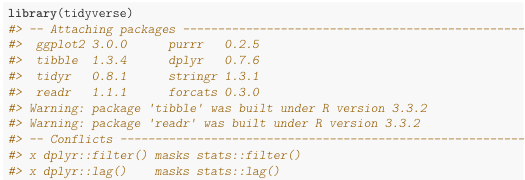
\includegraphics{~/Desktop/lecture8/tidyverse.png}\\
- For the purpose of this lecture, we will just need to load
\textbf{library(readr)}

\end{frame}

\begin{frame}[fragile]{\texttt{readr}}

No matter the flat file format you are working with, there are two
important steps for reading in data with \texttt{readr}:

\begin{enumerate}
\def\labelenumi{(\arabic{enumi})}
\item
  \textbf{a function to parse the file (read\_csv)}
\item
  \textbf{column specification}
\end{enumerate}

\textbf{Talk about readr (tidyverse), Notes from the reading, Notes from
other sources}

\end{frame}

\begin{frame}[fragile]{\texttt{readr\ functions}}

\textbf{readr's} (tidyverse) functions

\begin{longtable}[]{@{}ll@{}}
\toprule
\textbf{Format} & \textbf{Function}\tabularnewline
\midrule
\endhead
Comma-separated values (csv) & \texttt{read\_csv}\tabularnewline
Semicolon separated files & \texttt{read\_csv2}\tabularnewline
Tab-separated values (tsv) & \texttt{read\_tsv}\tabularnewline
Any delimiter & \texttt{read\_delim}\tabularnewline
Fixed width files & \texttt{read\_fwf}\tabularnewline
Text-formated data (txt) & \texttt{read\_table}\tabularnewline
Web log files & \texttt{read\_log}\tabularnewline
\bottomrule
\end{longtable}

\textbf{What type of data could be read in}

\end{frame}

\begin{frame}[fragile]{\texttt{readr\ column\ specification}}

\texttt{readr} is pretty good at guessing each column's data type
(e.g.~character, double, etc.), however it is good practice to manually
specify the data type for each column.

\begin{Shaded}
\begin{Highlighting}[]
\NormalTok{mtcars <-}\StringTok{ }\KeywordTok{read_csv}\NormalTok{(}\KeywordTok{readr_example}\NormalTok{(}\StringTok{"mtcars.csv"}\NormalTok{))}
\CommentTok{#> Parsed with column specification:}
\CommentTok{#> cols(}
\CommentTok{#>   mpg = col_double(),}
\CommentTok{#>   cyl = col_integer(),}
\CommentTok{#>   disp = col_double(),}
\CommentTok{#>   hp = col_integer(),}
\CommentTok{#>   drat = col_double(),}
\CommentTok{#>   wt = col_double(),}
\CommentTok{#>   qsec = col_double(),}
\CommentTok{#>   vs = col_integer(),}
\CommentTok{#>   am = col_integer(),}
\CommentTok{#>   gear = col_integer(),}
\CommentTok{#>   carb = col_integer()}
\CommentTok{#> )}
\end{Highlighting}
\end{Shaded}

\end{frame}

\begin{frame}[fragile]{\texttt{readr\ column\ specification}}

The output of the previous example shows us the column specification of
the variables in the data. This is important because we could manually
change column specification if we do not like readr's guess.

\begin{Shaded}
\begin{Highlighting}[]
\NormalTok{mtcars <-}\StringTok{ }\KeywordTok{read_csv}\NormalTok{(}\KeywordTok{readr_example}\NormalTok{(}\StringTok{"mtcars.csv"}\NormalTok{), }\DataTypeTok{col_types =} 
  \KeywordTok{cols}\NormalTok{(}
    \DataTypeTok{mpg =} \KeywordTok{col_double}\NormalTok{(),}
    \DataTypeTok{cyl =} \KeywordTok{col_integer}\NormalTok{(),}
    \DataTypeTok{disp =} \KeywordTok{col_double}\NormalTok{(),}
    \DataTypeTok{hp =} \KeywordTok{col_integer}\NormalTok{(),}
    \DataTypeTok{drat =} \KeywordTok{col_double}\NormalTok{(),}
    \DataTypeTok{vs =} \KeywordTok{col_integer}\NormalTok{(),}
    \DataTypeTok{wt =} \KeywordTok{col_double}\NormalTok{(),}
    \DataTypeTok{qsec =} \KeywordTok{col_double}\NormalTok{(),}
    \DataTypeTok{am =} \KeywordTok{col_integer}\NormalTok{(),}
    \DataTypeTok{gear =} \KeywordTok{col_integer}\NormalTok{(),}
    \DataTypeTok{carb =} \KeywordTok{col_integer}\NormalTok{()}
\NormalTok{  )}
\NormalTok{)}
\end{Highlighting}
\end{Shaded}

\end{frame}

\begin{frame}{\texttt{readr} features}

\textbf{skip}:\\
\textbf{comment}:\\
\textbf{col\_names}:

\end{frame}

\begin{frame}[fragile]{\texttt{readr} demonstration csv}

\texttt{readr} automatically treats the first line of data as column
names.

\begin{Shaded}
\begin{Highlighting}[]
\KeywordTok{read_csv}\NormalTok{(}\StringTok{"column 1, column 2, column 3}
\StringTok{         1,2,3}
\StringTok{         4,5,6"}
\NormalTok{         )}
\CommentTok{#> # A tibble: 2 x 3}
\CommentTok{#>   `column 1` `column 2` `column 3`}
\CommentTok{#>        <int>      <int>      <int>}
\CommentTok{#> 1          1          2          3}
\CommentTok{#> 2          4          5          6}
\end{Highlighting}
\end{Shaded}

There are instances where you may want to tell R from what line to begin
reading in data.

\end{frame}

\begin{frame}[fragile]{\texttt{readr} demonstration csv}

Notice the example below. The first two lines are comments about the
data. We would need to use \textbf{skip = n} to skip n lines.

\begin{Shaded}
\begin{Highlighting}[]
\KeywordTok{read_csv}\NormalTok{(}\StringTok{"This file contains data on student charges for the acdemic year.}
\StringTok{         File name: IC2016_AY}
\StringTok{         a, b, c}
\StringTok{         1,2,3}
\StringTok{         4,5,6"}\NormalTok{, }\DataTypeTok{skip =} \DecValTok{2}
\NormalTok{         )}
\CommentTok{#> # A tibble: 2 x 3}
\CommentTok{#>       a     b     c}
\CommentTok{#>   <int> <int> <int>}
\CommentTok{#> 1     1     2     3}
\CommentTok{#> 2     4     5     6}
\end{Highlighting}
\end{Shaded}

\end{frame}

\begin{frame}[fragile]{\texttt{readr} demonstration csv}

We could also tell R to drop lines we specify as comments. With
\textbf{comment = n}

\begin{Shaded}
\begin{Highlighting}[]
\KeywordTok{read_csv}\NormalTok{(}\StringTok{"# This file contains data on student charges for the acdemic year.}
\StringTok{         a, b, c}
\StringTok{         1,2,3}
\StringTok{         4,5,6"}\NormalTok{, }\DataTypeTok{comment =} \StringTok{"#"}
\NormalTok{         )}
\CommentTok{#> # A tibble: 2 x 3}
\CommentTok{#>       a     b     c}
\CommentTok{#>   <int> <int> <int>}
\CommentTok{#> 1     1     2     3}
\CommentTok{#> 2     4     5     6}
\end{Highlighting}
\end{Shaded}

\begin{Shaded}
\begin{Highlighting}[]
\KeywordTok{read_csv}\NormalTok{(}\StringTok{"* This file contains data on student charges for the acdemic year.}
\StringTok{         a, b, c}
\StringTok{         1,2,3}
\StringTok{         4,5,6"}\NormalTok{, }\DataTypeTok{comment =} \StringTok{"*"}
\NormalTok{         )}
\CommentTok{#> # A tibble: 2 x 3}
\CommentTok{#>       a     b     c}
\CommentTok{#>   <int> <int> <int>}
\CommentTok{#> 1     1     2     3}
\CommentTok{#> 2     4     5     6}
\end{Highlighting}
\end{Shaded}

\end{frame}

\begin{frame}[fragile]{\texttt{readr} column names}

We could tell R there are no column names with \textbf{col\_names =
FALSE} or we could manually give R column names with \textbf{col\_names
= c(``'', ``'', ``'')}

\begin{Shaded}
\begin{Highlighting}[]
\KeywordTok{read_csv}\NormalTok{(}\StringTok{"1,2,3}
\StringTok{         4,5,6"}\NormalTok{, }\DataTypeTok{col_names =} \OtherTok{FALSE}
\NormalTok{         )}
\CommentTok{#> # A tibble: 2 x 3}
\CommentTok{#>      X1    X2    X3}
\CommentTok{#>   <int> <int> <int>}
\CommentTok{#> 1     1     2     3}
\CommentTok{#> 2     4     5     6}
\end{Highlighting}
\end{Shaded}

\begin{Shaded}
\begin{Highlighting}[]
\KeywordTok{read_csv}\NormalTok{(}\StringTok{"1,2,3}
\StringTok{         4,5,6"}\NormalTok{, }\DataTypeTok{col_names =} \KeywordTok{c}\NormalTok{(}\StringTok{"column 1"}\NormalTok{, }\StringTok{"column 2"}\NormalTok{, }\StringTok{"column 3"}\NormalTok{)}
\NormalTok{         )}
\CommentTok{#> # A tibble: 2 x 3}
\CommentTok{#>   `column 1` `column 2` `column 3`}
\CommentTok{#>        <int>      <int>      <int>}
\CommentTok{#> 1          1          2          3}
\CommentTok{#> 2          4          5          6}
\end{Highlighting}
\end{Shaded}

\end{frame}

\begin{frame}{\texttt{readr} Student exercise}

\begin{itemize}
\tightlist
\item
  Get in your homework groups\\
\item
  Create a 3x3 tibble like the examples above
  (e.g.~read\_csv(``a,b,c\ldots{}.'')), treating the first line as
  column names\\
\item
  Now on the first line add a sentence\\
\item
  This time add a special character ( *, \#, ! ) at the beginning of the
  sentence and indicate it is a comment\\
\item
  Delete the sentence and column names (should have a 2x2 tibble) and
  manually tell R column names
\end{itemize}

\end{frame}

\begin{frame}[fragile]{\texttt{readr} demonstration csv}

\textbf{NOT SURE IF TO MAKE THIS A DEMONSTRATION WHERE STUDENTS FOLLOW
ALONG OR ANOTHER STUDENT EXERCISE}\\
\textbf{Tying it all together}

Use \texttt{read\_csv()} function from \texttt{readr} to import csv
dataset into R without column specification. Follow along on your
computers.

\begin{Shaded}
\begin{Highlighting}[]
\CommentTok{#ipeds_ay <- read_csv(file="../ic2017ay_small.csv")}
\end{Highlighting}
\end{Shaded}

Notice tuition and fee columns are read in as character type.

\end{frame}

\begin{frame}[fragile]{\texttt{readr} demonstration csv}

Use \texttt{read\_csv()} function from \texttt{readr} to import csv
dataset into R with column specification \textbf{{[}Would it be better
to change to integer or double?{]}}

\begin{Shaded}
\begin{Highlighting}[]
\CommentTok{# \{ipeds_ay <- read_csv("../ic2017ay_small.csv", col_types = }
\CommentTok{#  cols(}
\CommentTok{#    unitid = col_integer(),}
\CommentTok{#    tuition1 = col_integer(),}
\CommentTok{#    fee1 = col_integer(),}
 \CommentTok{#   hrchg1 = col_integer(),}
 \CommentTok{#   tuition2 = col_integer(),}
 \CommentTok{#   fee2 = col_integer(),}
 \CommentTok{#   hrchg2 = col_integer(),}
 \CommentTok{#   tuition3 = col_integer(),}
 \CommentTok{#   fee3 = col_integer(),}
 \CommentTok{#   hrchg3 = col_integer()}
 \CommentTok{# )}
\CommentTok{#) # \}}
\end{Highlighting}
\end{Shaded}

\end{frame}

\begin{frame}[fragile]{\texttt{readr\ Running\ into\ errors}}

\begin{enumerate}
\def\labelenumi{\arabic{enumi}.}
\tightlist
\item
  Make sure you have downloaded and saved flat file\\
\item
  Make sure to know the file path of where data is downloaded or saved
  (\textasciitilde{}/Desktop/educ263/data)
\item
  Make sure you set your working \textbf{\texttt{setwd()}} directory in
  R. To check your current working directory type
  \textbf{\texttt{getwd()}} in console.
\end{enumerate}

\end{frame}

\section{\texorpdfstring{\texttt{haven}
package}{haven package}}\label{haven-package}

\begin{frame}[fragile]{\texttt{haven}}

Recap from lecture 5

\href{https://haven.tidyverse.org/}{\texttt{haven}} is part of
\textbf{tidyverse}, which enables users to import and export data from
the following statistical packages:

\begin{itemize}
\tightlist
\item
  SAS
\item
  SPSS
\item
  Stata\\[2\baselineskip]
\end{itemize}

Similar to \texttt{readr}, we could load the entire
\textbf{library(tidyverse)} package to get \texttt{haven}. For the
purpose of this lecture, we will just need to load
\textbf{library(haven)}.

\end{frame}

\begin{frame}[fragile]{\texttt{haven\ functions}}

\textbf{haven's} (tidyverse) functions

\begin{longtable}[]{@{}ll@{}}
\toprule
\textbf{Format} & \textbf{Function}\tabularnewline
\midrule
\endhead
SPSS & \texttt{read\_sav}\tabularnewline
SAS & \texttt{read\_sas}\tabularnewline
Stata & \texttt{read\_dta}\tabularnewline
\bottomrule
\end{longtable}

\end{frame}

\begin{frame}[fragile]{\texttt{haven} read and write Stata arguments}

\texttt{read\_dta(file,\ encoding\ =\ NULL)}\\
\texttt{write\_data(data,\ path,\ version\ =\ 14)}

Arguments\\
- file: file path to data\\
- encoding: files prior to Stata 14 did not declare text encoding, files
after Stata 14 do not need to declare encoding value\\
- data: data frame to save (write)\\
- path: file path to where data will be saved\\
- version: file version

\href{https://haven.tidyverse.org/reference/read_dta.html}{Link}

\end{frame}

\begin{frame}[fragile]{\texttt{haven} read and write Stata example}

Use \texttt{read\_dta()} function from \texttt{haven} to import Stata
dataset into R

\begin{Shaded}
\begin{Highlighting}[]
\NormalTok{hsls <-}\StringTok{ }\KeywordTok{read_dta}\NormalTok{(}\StringTok{"~/Desktop/lecture8/hsls_sch_small.dta"}\NormalTok{, }\DataTypeTok{encoding=}\OtherTok{NULL}\NormalTok{)}

\CommentTok{# View data}
\KeywordTok{head}\NormalTok{(hsls)}
\KeywordTok{glimpse}\NormalTok{(hsls)}
\end{Highlighting}
\end{Shaded}

Use \texttt{write\_dta} function from \texttt{haven} to write State data

\begin{Shaded}
\begin{Highlighting}[]
\KeywordTok{write_dta}\NormalTok{(hsls, }\DataTypeTok{path =} \StringTok{"~/Desktop/lecture8/hsls_sch_small.dta"}\NormalTok{)}
\end{Highlighting}
\end{Shaded}

Student exercise Running into problems with variable/value labels?

\end{frame}

\section{\texorpdfstring{\texttt{readxl}
package}{readxl package}}\label{readxl-package}

\begin{frame}[fragile]{\texttt{readxl}}

The \href{https://readxl.tidyverse.org/}{\texttt{readxl}} package is
part of tidyverse, which is designed to easily read data from Excel and
into R.\\
- We could load \textbf{library(tidyverse)} if we wanted to load all
packages in tidyverse. For the purpose of this lecture, we just need to
load \textbf{library(readxl)}.

\end{frame}

\begin{frame}[fragile]{\texttt{readxl}}

\texttt{readxl} supports both .xls and .xlsx formats and is designed to
work with tabular data. It does not require dependencies-- making
installing and operating fairly simple.

\texttt{readxl} has several example files where we could use as
practice. The files include:

\begin{Shaded}
\begin{Highlighting}[]
\KeywordTok{readxl_example}\NormalTok{()}
\CommentTok{#>  [1] "clippy.xls"    "clippy.xlsx"   "datasets.xls"  "datasets.xlsx"}
\CommentTok{#>  [5] "deaths.xls"    "deaths.xlsx"   "geometry.xls"  "geometry.xlsx"}
\CommentTok{#>  [9] "type-me.xls"   "type-me.xlsx"}
\end{Highlighting}
\end{Shaded}

For now, lets use ``datasets.xlsx''

\begin{Shaded}
\begin{Highlighting}[]
\NormalTok{excel_example <-}\StringTok{ }\KeywordTok{readxl_example}\NormalTok{(}\StringTok{"datasets.xlsx"}\NormalTok{)}
\end{Highlighting}
\end{Shaded}

\end{frame}

\begin{frame}[fragile]{\texttt{readxl} features}

\begin{itemize}
\tightlist
\item
  \textbf{sheet}: \texttt{read\_excel}(excel file, sheet = ``sheet
  name'')
\item
  \textbf{n\_max}: \texttt{read\_excel}(excel file, n\_max = n)
\item
  \textbf{range}: \texttt{read\_excel}(excel file, range = ``A:D'')\\
\item
  \textbf{cell\_rows}: \texttt{read\_excel}(excel file, range =
  cell\_rows(1:n))
\item
  \textbf{cell\_cols}: \texttt{read\_excel}(excel file, range =
  cell\_cols(``A:D''))
\item
  \textbf{na}: \texttt{read\_excel}(excel file, na = ``n'')
\end{itemize}

\end{frame}

\begin{frame}[fragile]{\texttt{readxl} sheet}

\begin{Shaded}
\begin{Highlighting}[]
\CommentTok{#To view sheets in excel file}
\KeywordTok{excel_sheets}\NormalTok{(excel_example)}
\CommentTok{#> [1] "iris"     "mtcars"   "chickwts" "quakes"}
\end{Highlighting}
\end{Shaded}

\begin{Shaded}
\begin{Highlighting}[]
\NormalTok{xl_example <-}\StringTok{ }\KeywordTok{read_excel}\NormalTok{(excel_example, }\DataTypeTok{sheet =} \StringTok{"quakes"}\NormalTok{)}
\KeywordTok{head}\NormalTok{(xl_example)}
\CommentTok{#> # A tibble: 6 x 5}
\CommentTok{#>      lat   long depth   mag stations}
\CommentTok{#>    <dbl>  <dbl> <dbl> <dbl>    <dbl>}
\CommentTok{#> 1 -20.42 181.62   562   4.8       41}
\CommentTok{#> 2 -20.62 181.03   650   4.2       15}
\CommentTok{#> 3 -26.00 184.10    42   5.4       43}
\CommentTok{#> 4 -17.97 181.66   626   4.1       19}
\CommentTok{#> 5 -20.42 181.96   649   4.0       11}
\CommentTok{#> 6 -19.68 184.31   195   4.0       12}
\end{Highlighting}
\end{Shaded}

\end{frame}

\begin{frame}[fragile]{\texttt{readxl} n\_max}

\begin{Shaded}
\begin{Highlighting}[]
\KeywordTok{read_excel}\NormalTok{(excel_example, }\DataTypeTok{sheet =} \StringTok{"quakes"}\NormalTok{, }\DataTypeTok{n_max =} \DecValTok{3}\NormalTok{)}
\CommentTok{#> # A tibble: 3 x 5}
\CommentTok{#>      lat   long depth   mag stations}
\CommentTok{#>    <dbl>  <dbl> <dbl> <dbl>    <dbl>}
\CommentTok{#> 1 -20.42 181.62   562   4.8       41}
\CommentTok{#> 2 -20.62 181.03   650   4.2       15}
\CommentTok{#> 3 -26.00 184.10    42   5.4       43}
\end{Highlighting}
\end{Shaded}

\end{frame}

\begin{frame}[fragile]{\texttt{readxl} range}

\begin{Shaded}
\begin{Highlighting}[]
\KeywordTok{read_excel}\NormalTok{(excel_example, }\DataTypeTok{sheet =} \StringTok{"quakes"}\NormalTok{, }\DataTypeTok{range =} \StringTok{"C1:E4"}\NormalTok{)}
\CommentTok{#> # A tibble: 3 x 3}
\CommentTok{#>   depth   mag stations}
\CommentTok{#>   <dbl> <dbl>    <dbl>}
\CommentTok{#> 1   562   4.8       41}
\CommentTok{#> 2   650   4.2       15}
\CommentTok{#> 3    42   5.4       43}

\KeywordTok{read_excel}\NormalTok{(excel_example, }\DataTypeTok{sheet =} \StringTok{"quakes"}\NormalTok{, }\DataTypeTok{range =} \KeywordTok{cell_rows}\NormalTok{(}\DecValTok{1}\OperatorTok{:}\DecValTok{3}\NormalTok{))}
\CommentTok{#> # A tibble: 2 x 5}
\CommentTok{#>      lat   long depth   mag stations}
\CommentTok{#>    <dbl>  <dbl> <dbl> <dbl>    <dbl>}
\CommentTok{#> 1 -20.42 181.62   562   4.8       41}
\CommentTok{#> 2 -20.62 181.03   650   4.2       15}

\KeywordTok{head}\NormalTok{(}\KeywordTok{read_excel}\NormalTok{(excel_example, }\DataTypeTok{sheet =} \StringTok{"quakes"}\NormalTok{, }\DataTypeTok{range =} \KeywordTok{cell_cols}\NormalTok{(}\StringTok{"A:C"}\NormalTok{)))}
\CommentTok{#> # A tibble: 6 x 3}
\CommentTok{#>      lat   long depth}
\CommentTok{#>    <dbl>  <dbl> <dbl>}
\CommentTok{#> 1 -20.42 181.62   562}
\CommentTok{#> 2 -20.62 181.03   650}
\CommentTok{#> 3 -26.00 184.10    42}
\CommentTok{#> 4 -17.97 181.66   626}
\CommentTok{#> 5 -20.42 181.96   649}
\CommentTok{#> 6 -19.68 184.31   195}
\CommentTok{# using head() to only view first 6 rows }
\end{Highlighting}
\end{Shaded}

\end{frame}

\begin{frame}[fragile]{\texttt{readxl} na}

\begin{Shaded}
\begin{Highlighting}[]
\KeywordTok{read_excel}\NormalTok{(excel_example, }\DataTypeTok{sheet =} \StringTok{"quakes"}\NormalTok{, }\DataTypeTok{na =} \StringTok{"-20.42"}\NormalTok{)}
\CommentTok{#> # A tibble: 1,000 x 5}
\CommentTok{#>       lat   long depth   mag stations}
\CommentTok{#>     <dbl>  <dbl> <dbl> <dbl>    <dbl>}
\CommentTok{#>  1     NA 181.62   562   4.8       41}
\CommentTok{#>  2 -20.62 181.03   650   4.2       15}
\CommentTok{#>  3 -26.00 184.10    42   5.4       43}
\CommentTok{#>  4 -17.97 181.66   626   4.1       19}
\CommentTok{#>  5     NA 181.96   649   4.0       11}
\CommentTok{#>  6 -19.68 184.31   195   4.0       12}
\CommentTok{#>  7 -11.70 166.10    82   4.8       43}
\CommentTok{#>  8 -28.11 181.93   194   4.4       15}
\CommentTok{#>  9 -28.74 181.74   211   4.7       35}
\CommentTok{#> 10 -17.47 179.59   622   4.3       19}
\CommentTok{#> # ... with 990 more rows}
\end{Highlighting}
\end{Shaded}

\end{frame}

\begin{frame}[fragile]{\texttt{readxl} Student exercise}

\textbf{Save data} - Download and save Federal Student Financial Aid
Data\\
- Read in data using \texttt{readxl} function\\
- Read in first four rows (n\_max) - Read in column Names to column
State \textbf{hint} \texttt{cell\_cols} - Set value ``A'' to missing
(na) \textbf{note} : you need to investigate in detail before setting
anything to missing

\end{frame}

\begin{frame}[fragile]{\texttt{readxl} Running into problems}

\begin{enumerate}
\def\labelenumi{\arabic{enumi}.}
\tightlist
\item
  Make sure you have downloaded and saved excel file\\
\item
  Make sure to know the file path of where data is downloaded or saved
  (\textasciitilde{}/Desktop/educ263/data)
\item
  Make sure you set your working \textbf{\texttt{setwd()}} directory in
  R. To check your current working directory type
  \textbf{\texttt{getwd()}} in console.\\
\item
  Make sure to choose the correct sheet (if applicable)\\
\item
  Pay attention to column names when setting range
\end{enumerate}

\end{frame}

\section{Downloading data from web}\label{downloading-data-from-web}

\begin{frame}{Downloading data from web}

Could save time and reduce the steps of downloading, saving, and reading
in data, by reading in data directly from the web.\\
- note that not all packages will work downloading data from web
(read\_excel)

For example, rather than downloading ipeds data and saving it in a
folder, we could download the data directly from the web.

\end{frame}

\begin{frame}{Downloading data from web example using Raj Chetty data}

\begin{enumerate}
\def\labelenumi{\arabic{enumi}.}
\tightlist
\item
  Follow this \href{http://www.equality-of-opportunity.org/data/}{link}
  and under the ``Mobility Report Cards\ldots{}'' tab select ``click to
  view data''.\\
\item
  Choose ``Online Data Table 1''
\item
  Right click and copy link address for ``Excel'' (Note: it is actually
  a csv file)
\end{enumerate}

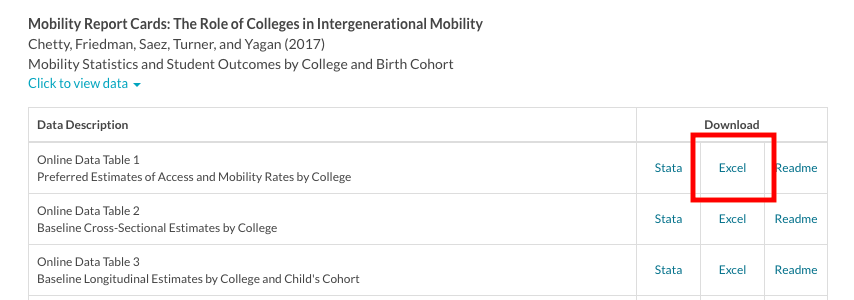
\includegraphics{~/Desktop/lecture8/mrc_table1.png}~

\end{frame}

\begin{frame}[fragile]{Downloading data from web}

{[}FIX OUTPUT (CUTTING OFF){]}

\begin{Shaded}
\begin{Highlighting}[]
\CommentTok{#Paste url to excel "csv" file}
\NormalTok{data_url <-}\StringTok{ "http://www.equality-of-opportunity.org/data/college/mrc_table1.csv"}

\CommentTok{#Download data and read in using read_csv (readr)}
\NormalTok{mrc <-}\StringTok{ }\KeywordTok{read_csv}\NormalTok{(data_url)}

\CommentTok{#View first 4 rows and 4 columns }
\NormalTok{mrc[}\DecValTok{1}\OperatorTok{:}\DecValTok{4}\NormalTok{, }\DecValTok{1}\OperatorTok{:}\DecValTok{4}\NormalTok{]}
\CommentTok{#> # A tibble: 4 x 4}
\CommentTok{#>   super_opeid                                         name   czname state}
\CommentTok{#>         <int>                                        <chr>    <chr> <chr>}
\CommentTok{#> 1        2665 Vaughn College Of Aeronautics And Technology New York    NY}
\CommentTok{#> 2        7273               CUNY Bernard M. Baruch College New York    NY}
\CommentTok{#> 3        2688              City College Of New York - CUNY New York    NY}
\CommentTok{#> 4        7022                          CUNY Lehman College New York    NY}
\end{Highlighting}
\end{Shaded}

\end{frame}

\begin{frame}[fragile]{Downloading data from web}

Alternative approach

\begin{Shaded}
\begin{Highlighting}[]
\CommentTok{#Download data and read in link directly using read_csv (readr)}
\NormalTok{mrc <-}\StringTok{ }\KeywordTok{read_csv}\NormalTok{(}\StringTok{"http://www.equality-of-opportunity.org/data/college/mrc_table1.csv"}\NormalTok{)}
\CommentTok{#> Parsed with column specification:}
\CommentTok{#> cols(}
\CommentTok{#>   super_opeid = col_integer(),}
\CommentTok{#>   name = col_character(),}
\CommentTok{#>   czname = col_character(),}
\CommentTok{#>   state = col_character(),}
\CommentTok{#>   par_median = col_integer(),}
\CommentTok{#>   k_median = col_integer(),}
\CommentTok{#>   par_q1 = col_double(),}
\CommentTok{#>   par_top1pc = col_double(),}
\CommentTok{#>   kq5_cond_parq1 = col_double(),}
\CommentTok{#>   ktop1pc_cond_parq1 = col_double(),}
\CommentTok{#>   mr_kq5_pq1 = col_double(),}
\CommentTok{#>   mr_ktop1_pq1 = col_double(),}
\CommentTok{#>   trend_parq1 = col_double(),}
\CommentTok{#>   trend_bottom40 = col_double(),}
\CommentTok{#>   count = col_double()}
\CommentTok{#> )}

\CommentTok{#View first 4 rows and 4 columns }
\NormalTok{mrc[}\DecValTok{1}\OperatorTok{:}\DecValTok{4}\NormalTok{, }\DecValTok{1}\OperatorTok{:}\DecValTok{4}\NormalTok{]}
\CommentTok{#> # A tibble: 4 x 4}
\CommentTok{#>   super_opeid                                         name   czname state}
\CommentTok{#>         <int>                                        <chr>    <chr> <chr>}
\CommentTok{#> 1        2665 Vaughn College Of Aeronautics And Technology New York    NY}
\CommentTok{#> 2        7273               CUNY Bernard M. Baruch College New York    NY}
\CommentTok{#> 3        2688              City College Of New York - CUNY New York    NY}
\CommentTok{#> 4        7022                          CUNY Lehman College New York    NY}
\end{Highlighting}
\end{Shaded}

\end{frame}

\begin{frame}{Problems downloading data (zip files) using IPEDS}

\begin{enumerate}
\def\labelenumi{\arabic{enumi}.}
\tightlist
\item
  Follow this \href{https://nces.ed.gov/ipeds/use-the-data}{link} and
  under the ``Survey Data'' tab select ``Complete data files''.\\
\item
  Choose ``All years'' and ``All surveys'' and click continue\\
\item
  Right click and copy link address for ``IC2017\_AY''
\end{enumerate}

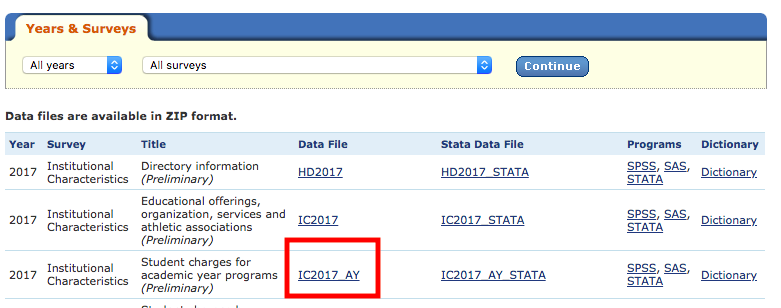
\includegraphics{~/Desktop/lecture8/ic2017_ay.png}~

\end{frame}

\begin{frame}[fragile]{Downloading data (zip files) using IPEDS}

\begin{Shaded}
\begin{Highlighting}[]
\CommentTok{# Paste url and read in using read_csv}
\CommentTok{# What happens when you try reading in this zip file? }
\CommentTok{#ic2017_ay <- read_csv("https://nces.ed.gov/ipeds/datacenter/data/IC2017_AY.zip")}

\CommentTok{# Need to download file first to unzip}
\end{Highlighting}
\end{Shaded}

\end{frame}

\begin{frame}[fragile]{Downloading data (zip files) using IPEDS}

\begin{Shaded}
\begin{Highlighting}[]
\CommentTok{#Set path to where data will be saved}
\NormalTok{path <-}\StringTok{ "~/Desktop/lecture8/ic2017_ay.csv"}
\CommentTok{#download file and pa}
\KeywordTok{download.file}\NormalTok{(}\StringTok{"https://nces.ed.gov/ipeds/datacenter/data/IC2017_AY.zip"}\NormalTok{, }\DataTypeTok{destfile =}\NormalTok{ path , }\DataTypeTok{mode =} \StringTok{'wb'}\NormalTok{)}
\CommentTok{#unzip zip file and keep original name}
\CommentTok{#unzip(zipfile = "ic2017_ay" , unzip = "unzip")}

\NormalTok{ic2017_ay <-}\StringTok{ }\KeywordTok{read_csv}\NormalTok{(path)}
\CommentTok{#> Parsed with column specification:}
\CommentTok{#> cols(}
\CommentTok{#>   `PK` = col_character()}
\CommentTok{#> )}
\CommentTok{#> Warning in rbind(names(probs), probs_f): number of columns of result is not}
\CommentTok{#> a multiple of vector length (arg 1)}
\CommentTok{#> Warning: 1680 parsing failures.}
\CommentTok{#> row # A tibble: 5 x 5 col     row              col  expected        actual expected   <int>            <chr>     <chr>         <chr> actual 1     1 "PK\textbackslash{}003\textbackslash{}004\textbackslash{}024"           embedded null file 2     2             <NA> 1 columns     3 columns row 3     3 "PK\textbackslash{}003\textbackslash{}004\textbackslash{}024"           embedded null col 4     3             <NA> 1 columns     3 columns expected 5     5             <NA> 1 columns     2 columns actual # ... with 1 more variables: file <chr>}
\CommentTok{#> ... ................. ... ................................................ ........ ................................................ ...... ................................................ .... ................................................ ... ................................................ ... ................................................ ........ ................................................ ...... .......................................}
\CommentTok{#> See problems(...) for more details.}
\end{Highlighting}
\end{Shaded}

\end{frame}

\begin{frame}{Student exercise}

\textbf{Tying it all together}

\begin{itemize}
\tightlist
\item
  Using everything we learned today read in a csv data file from the
  web\\
\item
  Go back to the ipeds data center
  \href{https://nces.ed.gov/ipeds/datacenter/DataFiles.aspx}{here}\\
\item
  Right click and copy the link address to a different data file
  (``HD2017'', ``EFFY2017'')\\
\item
  Make sure to download the link first (download.file) before reading
  in\\
\item
  Change column names to lowercase
\item
  Report dimensions of data\\
\item
  Create a subset of your data (filter, select, etc.)
\end{itemize}

\end{frame}

\section{Data sources (maybe)}\label{data-sources-maybe}

\end{document}
